%%%%%%%%%%%%%%%%%%%%%%%%%%%%%%%%%%%%%%%%%%%%%%%%%%%%%%%%%%%%%%%%%%%%%%%%%%%%%%%%%%%%%%%%%%%%%%%%%%%%%%%%%%%%%%%%%%%%%%%%%%%%%%%%%%%%%%%%%%%%%%%%%%%%%%%%%%%%%%%%%%%
% Written By Michael Brodskiy
% Class: Quantum Mechanics
% Professor: G. Fiete
%%%%%%%%%%%%%%%%%%%%%%%%%%%%%%%%%%%%%%%%%%%%%%%%%%%%%%%%%%%%%%%%%%%%%%%%%%%%%%%%%%%%%%%%%%%%%%%%%%%%%%%%%%%%%%%%%%%%%%%%%%%%%%%%%%%%%%%%%%%%%%%%%%%%%%%%%%%%%%%%%%%

\documentclass[12pt]{article} 
\usepackage{alphalph}
\usepackage[utf8]{inputenc}
\usepackage[russian,english]{babel}
\usepackage{titling}
\usepackage{amsmath}
\usepackage{float}
\usepackage{graphicx}
\usepackage{enumitem}
\usepackage{amssymb}
\usepackage[super]{nth}
\usepackage{everysel}
\usepackage{ragged2e}
\usepackage{geometry}
\usepackage{multicol}
\usepackage{fancyhdr}
\usepackage{cancel}
\usepackage{siunitx}
\usepackage{physics}
\usepackage{tikz}
\usepackage{mathdots}
\usepackage{yhmath}
\usepackage{cancel}
\usepackage{color}
\usepackage{array}
\usepackage{multirow}
\usepackage{gensymb}
\usepackage{tabularx}
\usepackage{extarrows}
\usepackage{booktabs}
\usepackage{lastpage}
\usetikzlibrary{fadings}
\usetikzlibrary{patterns}
\usetikzlibrary{shadows.blur}
\usetikzlibrary{shapes}

\geometry{top=1.0in,bottom=1.0in,left=1.0in,right=1.0in}
\newcommand{\subtitle}[1]{%
  \posttitle{%
    \par\end{center}
    \begin{center}\large#1\end{center}
    \vskip0.5em}%

}
\usepackage{hyperref}
\hypersetup{
colorlinks=true,
linkcolor=blue,
filecolor=magenta,      
urlcolor=blue,
citecolor=blue,
}


\title{Homework 1}
\date{\today}
\author{Michael Brodskiy\\ \small Professor: G. Fiete}

\begin{document}

\maketitle

\begin{enumerate}

  \item 

    \begin{enumerate}

      \item We can normalize each state vector by multiplying the coefficients of each state vector by some constant $c$. This gives us:

        \begin{enumerate}

          \item 

            $$|a|^2+|b|^2=1\Longrightarrow (3c)^2+(4c)^2=1$$

            This gives us:

            $$25c^2=1$$
            $$c^2=\frac{1}{25}$$
            $$c=\pm \frac{1}{5}$$

            Thus, we may normalize the first quantum state vector by writing:

            $$\boxed{\ket{\psi_1}=\frac{3}{5}\ket{+}+\frac{4}{5}\ket{-}}$$

          \item We continue with a similar approach to get:

            $$(c)^2+(2c)^2=1$$
            $$c^2=\frac{1}{5}$$
            $$c=\pm\frac{1}{\sqrt{5}}$$

            This gives us a normalized state vector:

            $$\boxed{\ket{\psi_2}=\frac{1}{\sqrt{5}}\ket{+}+\frac{2i}{\sqrt{5}}\ket{-}}$$

          \item We continue with the same procedure. Note that the magnitude of the exponential is 1, such that:

            $$(3c)^2+(c)^2=1$$
            $$c^2=10$$
            $$c=\pm\sqrt{10}$$

            This gives us:

            $$\boxed{\ket{\psi_3}=\frac{3}{\sqrt{10}}\ket{+}+\frac{e^{\frac{\pi i}{3}}}{\sqrt{10}}\ket{-}}$$

        \end{enumerate}

      \item We may write the probability expression as: $P_{\pm}=|\bra{\pm}{\ket{\psi}}|^2$

        \begin{enumerate}

          \item We use $a$ from the normalized state vector. Since we know that $\bra{+}\ket{\psi}=a$ and $\bra{-}\ket{\psi}=b$, we may get:

            $$P_+=a^2$$
            $$\boxed{P_+=\frac{9}{25}}$$
            $$P_-=b^2$$
            $$\boxed{P_-=\frac{16}{25}}$$

            We then need to find the probabilities in the $x$ and $y$ axis orientations. For the $S_x$ orientation, we know:

            $$S_x\Rightarrow \frac{1}{\sqrt{2}}(\ket{+}\pm \ket{-})$$

            This gives us:

            $$P_{+x}=\Big|\frac{1}{\sqrt{2}}(\bra{+}+\bra{-})\frac{1}{5}(3\ket{+}+4\ket{-})\Big|^2$$
            $$P_{+x}=\frac{1}{50}\Big|3\braket{+}+4\braket{-})\Big|^2$$
            $$\boxed{P_{+x}=\frac{49}{50}}$$

            Consequently, we write:

            $$\boxed{P_{-x}=1-\frac{49}{50}=\frac{1}{50}}$$

            Finally, we know that the $S_y$ orientation may be written as:

            $$S_y=\frac{1}{\sqrt{2}}(\ket{+}\pm i\ket{-})$$

            This gives us:

            $$P_{+y}=\Big|\frac{1}{\sqrt{2}}(\bra{+}+i\bra{-})\frac{1}{5}(3\ket{+}-4\ket{-})\Big|^2$$
            $$P_{+y}=\frac{1}{50}\Big|3\braket{+}-4i\braket{-}\Big|^2$$
            $$\boxed{P_{+y}=\frac{25}{50}=\frac{1}{2}}$$

            And, consequently, we get:

            $$\boxed{P_{-y}=1-\frac{25}{50}=\frac{1}{2}}$$

          \item Similarly, we take the coefficients to write:

            $$P_+=a^2$$
            $$\boxed{P_+=\frac{1}{5}}$$
            $$P_-=b^2$$
            $$\boxed{P_-=\frac{4}{5}}$$

            We then check the $S_x$ orientation to write:

            $$P_{+x}=\Big|\frac{1}{\sqrt{2}}(\bra{+}+\bra{-})\frac{1}{\sqrt{5}}(\ket{+}+2i\ket{-})\Big|^2$$
            $$P_{+x}=\frac{1}{10}\Big|\braket{+}+2i\braket{-}\Big|^2$$
            $$\boxed{P_{+x}=\frac{5}{10}=\frac{1}{2}}$$

            And, consequently:

            $$\boxed{P_{-x}=1-\frac{5}{10}=\frac{1}{2}}$$

            We then check the $S_y$ orientation to get:

            $$P_{+y}=\Big|\frac{1}{\sqrt{2}}(\bra{+}+i\bra{-})\frac{1}{\sqrt{5}}(\ket{+}-2i\ket{-})\Big|^2$$
            $$P_{+y}=\frac{1}{10}\Big|\braket{+}+2\braket{-}\Big|^2$$
            $$\boxed{P_{+y}=\frac{9}{10}}$$

            And, consequently:

            $$\boxed{P_{-y}=1-\frac{9}{10}=\frac{1}{10}}$$

          \item Finally, we find the last quantum state vector probabilities as:

            $$P_+=a^2$$
            $$\boxed{P_+=\frac{9}{10}}$$
            $$P_-=b^2$$
            $$\boxed{P_-=\frac{1}{10}}$$

            We then check the $S_x$ orientation:

            $$P_{+x}=\Big|\frac{1}{\sqrt{2}}(\bra{+}+\bra{-})\frac{1}{\sqrt{10}}(3\ket{+}+e^{\frac{\pi i}{3}}\ket{-})\Big|^2$$
            $$P_{+x}=\frac{1}{20}\Big|3\braket{+}+e^{\frac{\pi i}{3}}\braket{-}\Big|^2$$

            We may convert to rectangular to get:

            $$P_{+x}=\frac{1}{20}\Big|3+\left( \frac{1}{2}+\frac{\sqrt{3}}{2}i \right)\Big|^2$$
            $$P_{+x}=\frac{1}{20}\Big|\frac{7}{2}+\frac{\sqrt{3}}{2}i \Big|^2$$
            $$\boxed{P_{+x}=\frac{52}{80}=\frac{13}{20}}$$

            Consequently, we write:

            $$\boxed{P_{-x}=1-\frac{13}{20}=\frac{7}{20}}$$

            Finally, we check the $S_y$ orientation to get:

            $$P_{+y}=\Big|\frac{1}{\sqrt{2}}(\bra{+}-i\bra{-})\frac{1}{\sqrt{10}}(3\ket{+}+e^{\frac{\pi i}{3}}\ket{-})\Big|^2$$
            $$P_{+y}=\frac{1}{20}\Big|(\bra{+}-i\bra{-})\left( 3\ket{+}+\left( \frac{1}{2}+\frac{\sqrt{3}}{2}i \right)\ket{-} \right)\Big|^2$$
            $$\boxed{P_{+y}=\frac{10+3\sqrt{3}}{20}}$$

            Consequently, we get:

            $$\boxed{P_{-y}=1-\frac{10+3\sqrt{3}}{20}}=\frac{10-3\sqrt{3}}{20}$$

        \end{enumerate}

      \item We can write the matrix forms of the up and down vectors as:

        $$\ket{+}=\left( \begin{matrix} 1\\ 0\end{matrix} \right)\quad\text{ and }\quad\ket{-}=\left( \begin{matrix} 0\\ 1\end{matrix} \right)$$

        \begin{enumerate}

          \item Using the above, we may multiply to write:

            $$\ket{\psi_1}=\frac{3}{5}\left( \begin{matrix}1\\0\end{matrix} \right)+\frac{4}{5}\left( \begin{matrix} 0\\1\end{matrix} \right)$$
            $$\boxed{\ket{\psi_1}=\frac{1}{5}\left( \begin{matrix}3\\4\end{matrix} \right)}$$

          \item We use the same strategy to write:

            $$\ket{\psi_2}=\frac{1}{\sqrt{5}}\left( \begin{matrix}1\\0\end{matrix} \right)+\frac{2i}{\sqrt{5}}\left( \begin{matrix} 0\\1\end{matrix} \right)$$
            $$\boxed{\ket{\psi_2}=\frac{1}{\sqrt{5}}\left( \begin{matrix} 1\\2i\end{matrix} \right)}$$

          \item For the final quantum state vector, let us rewrite in rectangular for easier understanding:

            $$\ket{\psi_3}=\frac{3}{\sqrt{10}}\ket{+}+\left( \frac{1}{2\sqrt{10}}+\frac{\sqrt{3}i}{2\sqrt{10}} \right)\ket{-}$$
            $$\ket{\psi_3}=\frac{3}{\sqrt{10}}\left( \begin{matrix}1\\0\end{matrix} \right)+\left( \frac{1}{2\sqrt{10}}+\frac{\sqrt{3}i}{2\sqrt{10}} \right)\left( \begin{matrix} 0\\1\end{matrix} \right)$$
            $$\boxed{\ket{\psi_3}=\frac{1}{2\sqrt{10}}\left( \begin{matrix} 6\\1+\sqrt{3}i\end{matrix} \right)}$$

        \end{enumerate}

      \item To find the probabilities in matrix form, we may multiply the matrix form of the quantum state vector with the respective 'up' or 'down' matrix form, and square the result

        \begin{enumerate}

          \item Using this, we may write:

            $$P_+=\left[\left( \dfrac{3}{5}\quad \dfrac{4}{5} \right)\left( \begin{matrix} 1\\ 0\end{matrix} \right)\right]^2$$
            $$P_+=\left[\frac{3}{5}\right]^2$$
            $$\boxed{P_+=\frac{9}{25}}$$
            $$\boxed{P_-=1-\frac{9}{25}=\frac{16}{25}}$$

            We then use the $S_x$ orientation to write:

            $$P_{+x}=\left[\left( \dfrac{3}{5\sqrt{2}}\quad \dfrac{4}{5\sqrt{2}} \right)\left( \begin{matrix} 1\\ 1\end{matrix} \right)\right]^2$$
            $$\boxed{P_{+x}=\frac{49}{50}}$$

            And, consequently, we get:

            $$\boxed{P_{-x}=\frac{1}{50}}$$

            Then we check the $S_y$ orientation:

            $$P_{+y}=\left[\left( \dfrac{3}{5\sqrt{2}}\quad \dfrac{4}{5\sqrt{2}} \right)\left( \begin{matrix} 1\\ -i\end{matrix} \right)\right]^2$$
            $$P_{+y}=\frac{1}{50}\left[\left( 7\quad -1\right)\left( \begin{matrix} 1\\ i\end{matrix} \right)\right]^2$$
            $$\boxed{P_{+y}=\frac{25}{50}=\frac{1}{2}}$$

            Consequently, we get:

            $$\boxed{P_{-y}=1-\frac{50}{100}=\frac{1}{2}}$$

          \item We repeat the same for the next quantum state function:

            $$P_+=\left[\frac{1}{\sqrt{5}}\left( 1 \quad 2i \right)\left( \begin{matrix} 1\\ 0\end{matrix} \right)\right]^2$$
            $$P_+=\left[\frac{1}{\sqrt{5}}\right]^2$$
            $$\boxed{P_+=\frac{1}{5}}$$
            $$\boxed{P_-=1-\frac{1}{5}=\frac{4}{5}}$$

            We then check the $S_x$ direction:

            $$P_{+x}=\frac{1}{10}\left[\left( 1 \quad 2i \right)\left( \begin{matrix} 1\\ 1\end{matrix} \right)\right]^2$$
            $$\boxed{P_{+x}=\frac{5}{10}=\frac{1}{2}}$$

            Consequently, we may find:

            $$\boxed{P_{-x}=1-\frac{5}{10}=\frac{1}{2}}$$

            Finally, we find the $S_y$ orientation probability:

            $$P_{+y}=\frac{1}{10}\left[\left( 1\quad 2i \right)\left( \begin{matrix} 1\\ -i\end{matrix} \right)\right]^2$$
            $$P_{+y}=\frac{1}{10}\left[3\right]^2$$
            $$\boxed{P_{+y}=\frac{9}{10}}$$

            Consequently, we get:

            $$\boxed{P_{-y}=1-\frac{9}{10}=\frac{1}{10}}$$

          \item 

            $$P_+=\left[\frac{1}{2\sqrt{10}}\left(6 \quad 1+\sqrt{3}i \right)\left( \begin{matrix} 1\\ 0\end{matrix} \right)\right]^2$$
            $$\boxed{P_+=\frac{36}{40}=\frac{9}{10}}$$
            $$\boxed{P_-=1-\frac{9}{10}=\frac{1}{10}}$$

            We then check the $S_x$ orientation probability:

            $$P_{+x}=\frac{1}{80}\left[\left( 6 \quad 1+\sqrt{3}i \right)\left( \begin{matrix} 1\\ 1\end{matrix} \right)\right]^2$$
            $$\boxed{P_{+x}=\frac{52}{80}=\frac{13}{20}}$$

            Consequently, we find:

            $$\boxed{P_{-x}=1-\frac{52}{80}=\frac{7}{20}}$$

            We then find the $S_y$ orientation:

            $$P_{+y}=\left[\frac{1}{2\sqrt{20}}\left( 6 \quad 1+\sqrt{3}i \right)\left( \begin{matrix} 1\\ -i\end{matrix} \right)\right]^2$$
            $$P_{+y}=\frac{1}{80}\left[\left( 6 +\sqrt{3} -i \right)\right]^2$$
            $$\boxed{P_{+y}=\frac{40+12\sqrt{3}}{80}=\frac{10+3\sqrt{3}}{20}}$$

            Consequently, we find:

            $$\boxed{P_{+y}=1-\frac{40+12\sqrt{3}}{80}=\frac{10-3\sqrt{3}}{20}}$$

            We may observe that whether bra-ket notation or matrix form is used, the probability remains the same.

        \end{enumerate}

    \end{enumerate}

  \item 

    \begin{enumerate}

      \item We know that the probability in the $S_z$ orientation for such a quantum state function is simply the squares of the coefficients. This gives us:

        $$P_+=a^2$$
        $$\boxed{P_+=\left(\frac{2}{\sqrt{13}}\right)^2=\frac{4}{13}}$$

        Consequently, we may find:

        $$P_-=b^2$$
        $$\boxed{P_-=\left(\frac{3}{\sqrt{13}}\right)^2=\frac{9}{13}}$$

      \item We may find the $S_x$ orientation by using matrix form. This will give us:

        $$\ket{\psi}=\frac{1}{\sqrt{13}}\left( \begin{matrix} 2\\ 3i \end{matrix}\right)$$

        We then multiply by the $S_x$ matrix:

        $$\ket{\pm}_x=\frac{1}{\sqrt{2}}\left( \begin{matrix} 1\\\pm1\end{matrix} \right)$$

        This gives us:

        $$P_{+x}=\frac{1}{26}\Big| (1\quad 1)\left( \begin{matrix} 2\\ 3i\end{matrix} \right)\Big|^2$$
        $$P_{+x}=\frac{1}{26}\Big| 2+3i\Big|^2$$
        $$\boxed{P_{+x}=\frac{13}{26}=\frac{1}{2}}$$

        Consequently, we find:

        $$\boxed{P_{-x}=1-\frac{13}{26}=\frac{1}{2}}$$

      \item The probabilities may be plotted as follows:

        \begin{figure}[H]
          \centering
          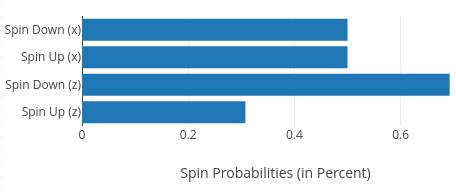
\includegraphics[width=.8\textwidth]{Figures/HW1-2c}
          \label{fig:1}
        \end{figure}

    \end{enumerate}

  \item We may observe that the results from (a) and (b) in part 2 are swapped in part (3)

    \begin{enumerate}

      \item Given that the orientation is towards the $x$ axis, we may write the state function in matrix as:

        $$\ket{\psi}=\frac{1}{\sqrt{2}}\left[ \frac{2}{\sqrt{13}}\left( \begin{matrix} 1\\1\end{matrix}\right) + \frac{3i}{\sqrt{13}}\left( \begin{matrix} 1\\-1\end{matrix} \right) \right]$$
        $$\ket{\psi}=\frac{1}{\sqrt{26}}\left( \begin{matrix} 2+3i\\2-3i\end{matrix} \right)$$

        We then multiply by the $S_z$ orientation to get:

        $$P_+=\frac{1}{26}\Big| \left( \begin{matrix} 2+3i\\2-3i\end{matrix} \right)(1\quad0)\Big|^2$$
        $$P_+=\frac{1}{26}\Big| 2+3i\Big|^2$$
        $$\boxed{P_+=\frac{13}{26}=\frac{1}{2}}$$

        Consequently, we may find:

        $$\boxed{P_-=1-\frac{13}{26}=\frac{1}{2}}$$

      \item We then use a similar process to find:

        $$P_{+x}=\frac{1}{52}\Big| \left( \begin{matrix} 2+3i\\2-3i\end{matrix} \right)(1\quad1)\Big|^2$$
        $$\boxed{P_{+x}=\frac{16}{52}=\frac{4}{13}}$$

        And, consequently:

        $$\boxed{P_{-x}=1-\frac{16}{52}=\frac{9}{13}}$$

      \item We may then re-plot to get:

        \begin{figure}[H]
          \centering
          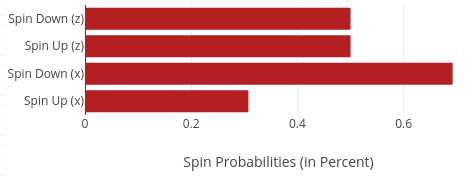
\includegraphics[width=.8\textwidth]{Figures/HW1-3c}
          \label{fig:2}
        \end{figure}

    \end{enumerate}

  \item 

    \begin{enumerate}

      \item First and foremost, we may observe that the $S_z$ probabilities are identical for each of the given quantum states. These probabilities are:

        $$\boxed{P_+=\left( \frac{4}{5} \right)^2=\frac{16}{25}}$$
        $$\boxed{P_-=\left( \frac{3}{5} \right)^2=\frac{9}{25}}$$

        We may then rewrite each state in terms of matrix form to get:

        $$\ket{\psi_1}\frac{1}{5}\left( \begin{matrix} 4\\3i \end{matrix} \right)$$
        $$\ket{\psi_2}\frac{1}{5}\left( \begin{matrix} 4\\-3i \end{matrix} \right)$$
        $$\ket{\psi_1}\frac{1}{5}\left( \begin{matrix} -4\\3i \end{matrix} \right)$$

        We can then calculate probabilities for the $S_x$ and $S_y$ orientations. Continuing, we check each wave function:

        \begin{enumerate}

          \item Function 1:

            We begin with $S_x$:

            $$P_{+x}=\frac{1}{50}\Big| (1\quad1)\left( \begin{matrix} 4\\3i \end{matrix} \right)\Big|^2$$
            $$P_{+x}=\frac{1}{50}\Big| (4+3i)\Big|^2$$
            $$\boxed{P_{+x}=\frac{1}{2}}$$

            Consequently, we write:

            $$\boxed{P_{-x}=\frac{1}{2}}$$

            We then check the $y$ orientation, which gives us:

            $$P_{+y}=\frac{1}{50}\Big| (1\quad -i)\left( \begin{matrix} 4\\3i \end{matrix} \right)\Big|^2$$
            $$\boxed{P_{+y}=\frac{49}{50}}$$

            Consequently, we may get:

            $$\boxed{P_{-y}=1-\frac{49}{50}=\frac{1}{50}}$$

          \item Function 2:

            We begin with $S_x$:

            $$P_{+x}=\frac{1}{50}\Big| (1\quad1)\left( \begin{matrix} 4\\-3i \end{matrix} \right)\Big|^2$$
            $$P_{+x}=\frac{1}{50}\Big| (4-3i)\Big|^2$$
            $$\boxed{P_{+x}=\frac{1}{2}}$$

            Consequently, we write:

            $$\boxed{P_{-x}=\frac{1}{2}}$$

            We then check the $y$ orientation, which gives us:

            $$P_{+y}=\frac{1}{50}\Big| (1\quad -i)\left( \begin{matrix} 4\\-3i \end{matrix} \right)\Big|^2$$
            $$\boxed{P_{+y}=\frac{1}{50}}$$

            Consequently, we may get:

            $$\boxed{P_{-y}=1-\frac{1}{50}=\frac{49}{50}}$$

          \item Function 3:

            $$P_{+x}=\frac{1}{50}\Big| (1\quad1)\left( \begin{matrix} -4\\3i \end{matrix} \right)\Big|^2$$
            $$P_{+x}=\frac{1}{50}\Big| (-4+3i)\Big|^2$$
            $$\boxed{P_{+x}=\frac{1}{2}}$$

            Consequently, we write:

            $$\boxed{P_{-x}=\frac{1}{2}}$$

            We then check the $y$ orientation, which gives us:

            $$P_{+y}=\frac{1}{50}\Big| (1\quad -i)\left( \begin{matrix} -4\+3i \end{matrix} \right)\Big|^2$$
            $$\boxed{P_{+y}=\frac{1}{50}}$$

            Consequently, we may get:

            $$\boxed{P_{-y}=1-\frac{1}{50}=\frac{49}{50}}$$

        \end{enumerate}

      \item We may observe that the $S_z$ and $S_x$ probabilities remained invariant. On the other hand, the $S_y$ probabilities were dependent on the phase; that is, for a $\pi/2$ change in phase, the probabilities switch (the up probability becomes the down probability and vice versa). We may observe that the probabilities are equivalent for $\ket{\psi_2}$ and $\ket{\psi_3}$.

    \end{enumerate}

\end{enumerate}

\end{document}

